% XCircuit output "Counter.tex" for LaTeX input from Counter.ps
\def\putbox#1#2#3#4{\makebox[0in][l]{\makebox[#1][l]{}\raisebox{\baselineskip}[0in][0in]{\raisebox{#2}[0in][0in]{\scalebox{#3}{#4}}}}}
\def\rightbox#1{\makebox[0in][r]{#1}}
\def\centbox#1{\makebox[0in]{#1}}
\def\topbox#1{\raisebox{-0.60\baselineskip}[0in][0in]{#1}}
\def\midbox#1{\raisebox{-0.20\baselineskip}[0in][0in]{#1}}
   \scalebox{0.5}{
   \normalsize
   \parbox{5.16667in}{
   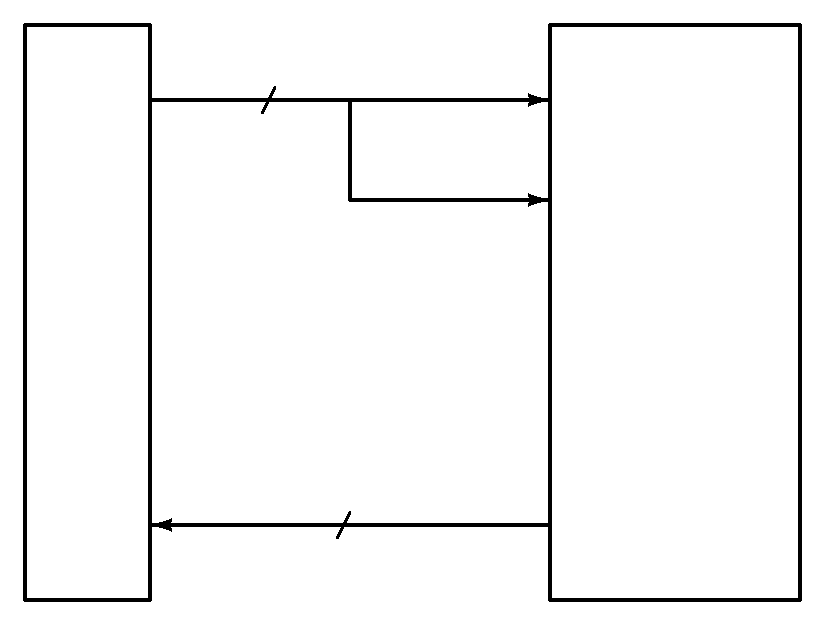
\includegraphics[scale=0.8]{Counter.eps}\\
   % translate x=672 y=512 scale 0.38
   \putbox{0.78in}{2.86in}{1.20}{\texttt{dut\_in[1:0]}}%
   \putbox{1.97in}{2.86in}{1.20}{\texttt{dut\_in[1]}}%
   \putbox{1.97in}{2.32in}{1.20}{\texttt{dut\_in[0]}}%
   \putbox{1.36in}{0.62in}{1.20}{\texttt{dut\_out[7:0]}}%
   \putbox{2.94in}{0.4in}{1.20}{\texttt{count}}%
   \putbox{2.94in}{2.65in}{1.20}{\texttt{reset}}%
   \putbox{2.94in}{2.1in}{1.20}{\texttt{clock}}%
   \putbox{0.35in}{1.16in}{1.20}{\rotatebox{-270}{Scan Chain}}%
   \putbox{3.2in}{1.4in}{1.20}{Counter}%
   } % close 'parbox'
   } % close 'scalebox'
   \vspace{-\baselineskip} % this is not necessary, but looks better
